
\begin{IEEEbiography}[{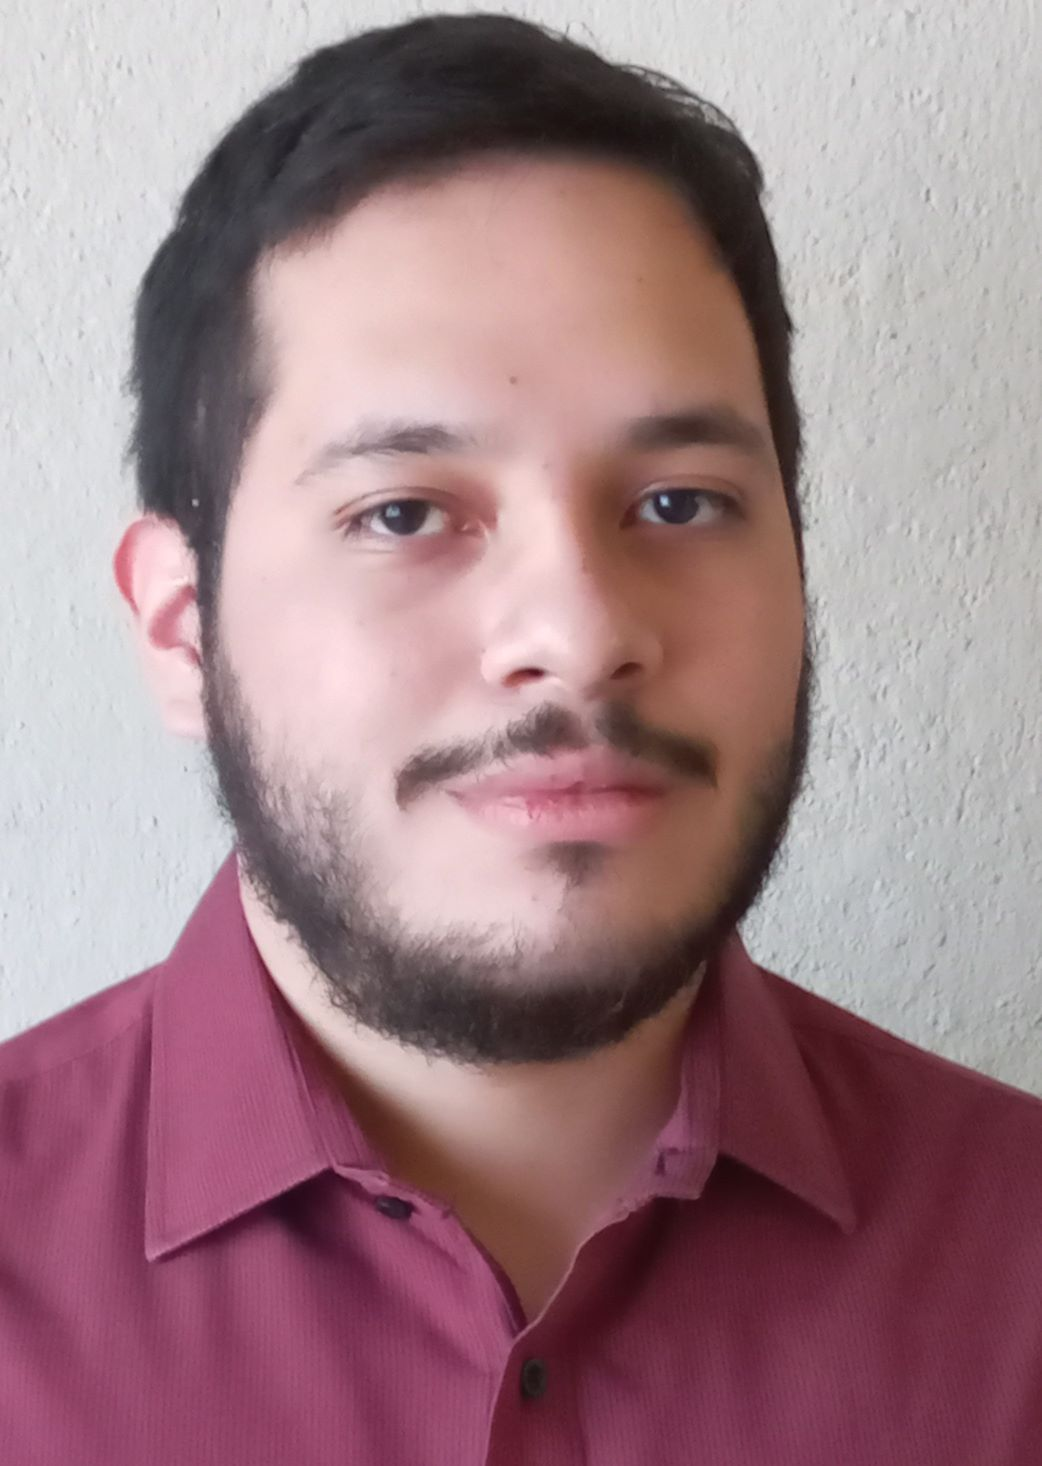
\includegraphics[width=1in,height=1.25in,clip,keepaspectratio]{Pictures/Daniel.jpg}}]{Daniel Mundo}
    He was born on May 16, 2001 in the capital city of Guatemala, he moved to Cobán at the age of 5, he lived and did most of his studies at San Francisco Javier de la Verapaz, until he returned to the capital city to complete his university studies at Universidad del Valle de Guatemala.
    \end{IEEEbiography}

\begin{IEEEbiography}[{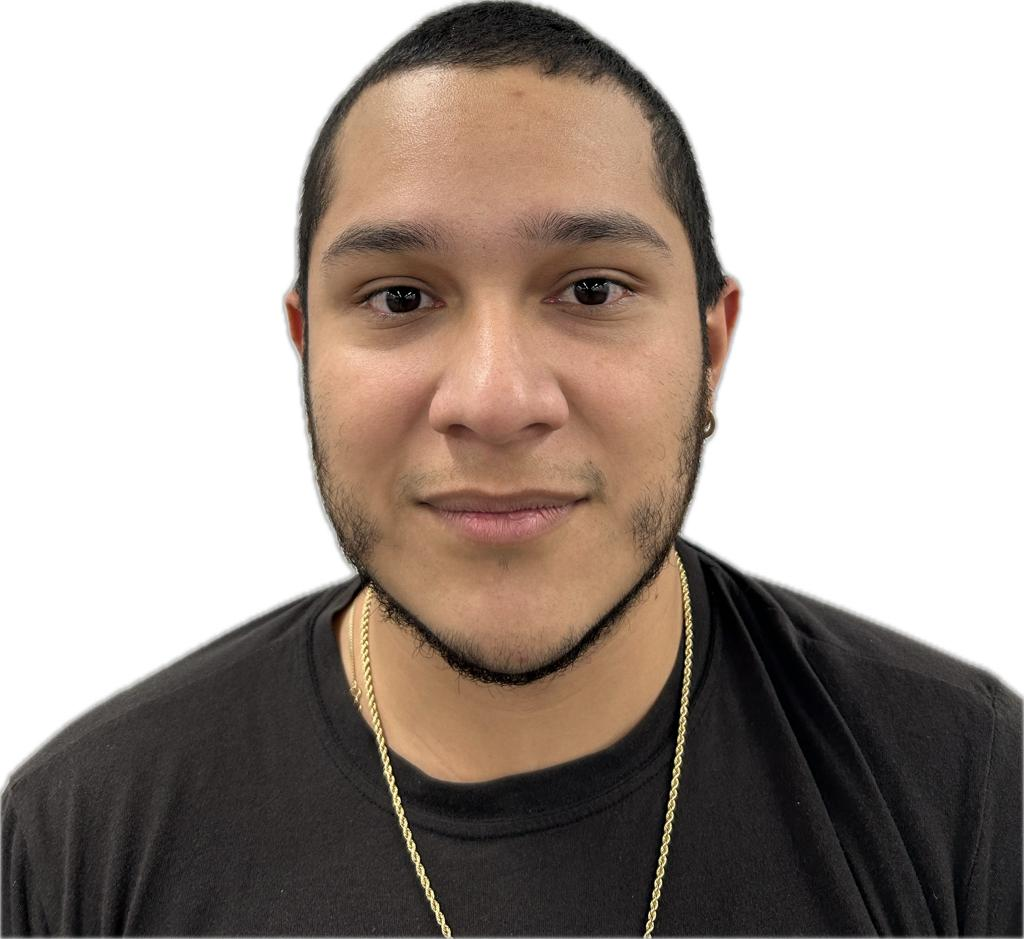
\includegraphics[width=1in,height=1.25in,clip,keepaspectratio]{Pictures/Julio.jpg}}]{Julio E. Lopez}
    was born in Guatemala city in 1999 April 20th. Lived in San Ignacio, Cayo Belize. Went to school at
    St. Andrews Primary school then, moved forward to Sacred heart High school to do 2 of
    his 4 years of high school then he moved out of his house to live on his own for the last
    two years of high school at the great and prestige St. Johns college where when graduated from
    arts and physics majors. Through all of his schooling he was a player in the St. Andrews, Sacred Heart school , And St Johns
    college basketball team. He is currently a student at Universidad del Valle de Guatemala on his last semester of electronic engineering.
\end{IEEEbiography}

\begin{IEEEbiography}[{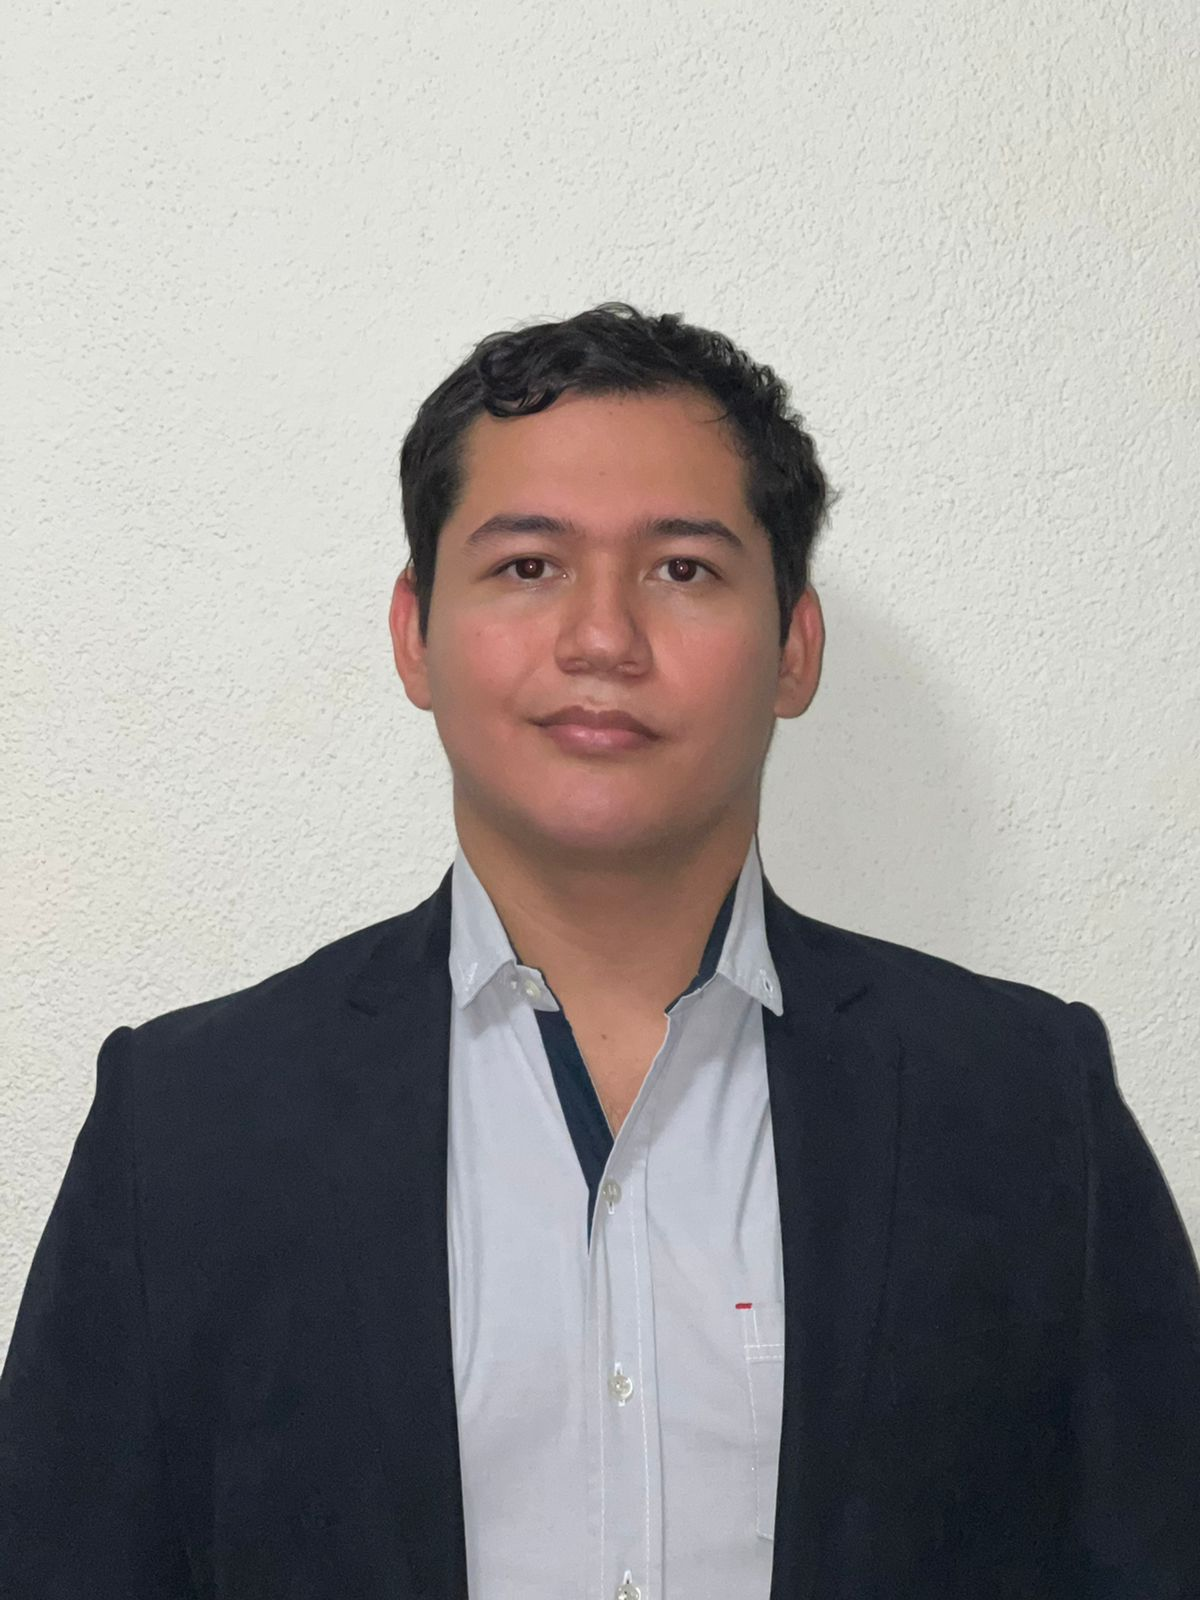
\includegraphics[width=1in,height=1.25in,clip,keepaspectratio]{Pictures/angel.jpg}}]{Angel Orellana}
    He was born on September 18, 2000 in the capital city of Guatemala
    he moved to Zacapa at the age of 7 and did most of his studies at the
    San Francisco Javier de Zacapa, at the age of 16 starts his high school studies at the
    Liceo La Salle Chiquimula, where he graduated in 2018, currently
    he is a final semester student of 
    electronic engineering at Universidad del Valle 
    de Guatemala. He has a passion for designing analog and digital circuits, 
    programming, and telecommunications.
\end{IEEEbiography}

\begin{IEEEbiography}[{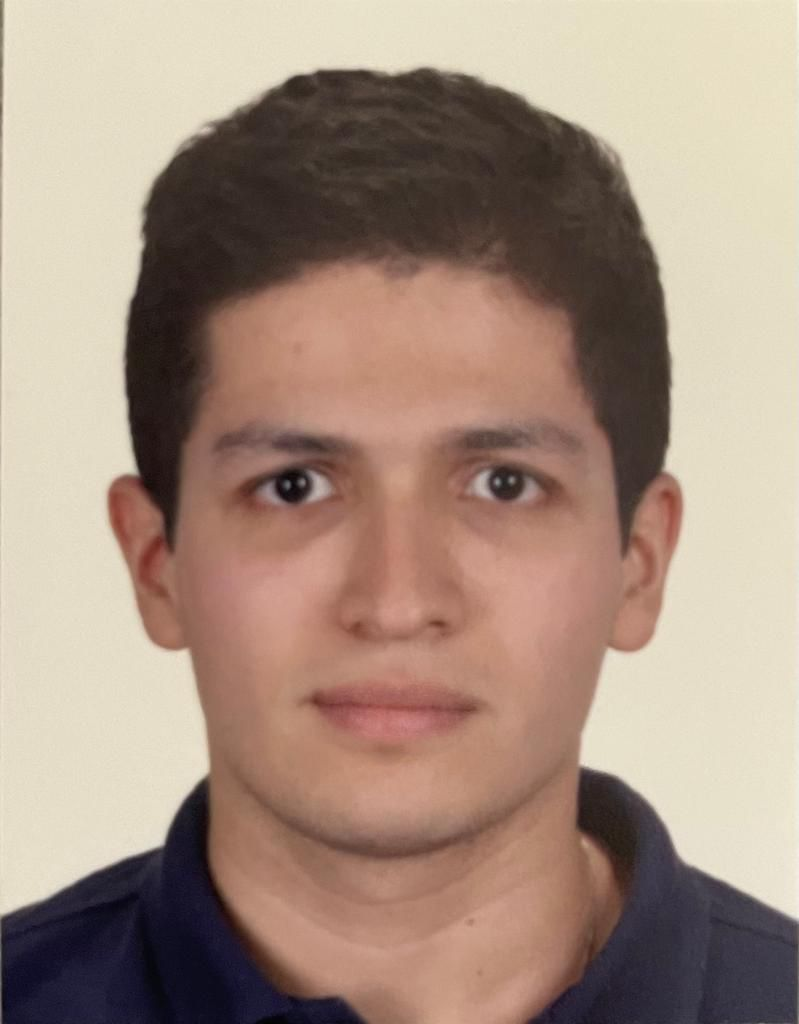
\includegraphics[width=1in,height=1.25in,clip,keepaspectratio]{Pictures/Noel.jpg}}]{Noel Prado}
    Born on September 30, 2000, in Guatemala City, Noel Prado completed his high school education at Centro Escolar El Roble. He is now in his final semester of Electronic Engineering at Universidad del Valle de Guatemala. Known for his passion for circuit design and VLSI, Noel Prado combines academic excellence with practical application in his field, positioning himself as a promising engineer in the making
\end{IEEEbiography}